\documentclass[11pt]{article}
\usepackage{worksheet_style}

% ---- Toggle: uncomment for filled version ----
%\worksheetfilledtrue
\begin{document}
\worksheetheader{10}{Directional Derivatives \& the Gradient}

\begin{background}
Partial derivatives measure change along the coordinate axes. But what if we want the rate of change in an arbitrary direction? The directional derivative answers this, and the gradient vector $\nabla f$ tells us the direction of fastest increase. The gradient is one of the most important objects in all of applied mathematics---it drives optimization, machine learning, physics, and engineering.
\end{background}

%=============================================================
\wsection{Notation Review}

-- We write vectors in bold: $\vect{x} = \vec{x_1, x_2}$ or $\vect{x} = \vec{x_1, x_2, x_3}$

-- A function $f\colon \R^n \to \R$ takes a vector input and returns a scalar

-- Partial derivatives: $f_x$, $f_y$, or $\frac{\partial f}{\partial x}$, $\frac{\partial f}{\partial y}$

%=============================================================
\wsection{The Directional Derivative}

\begin{defbox}{Directional Derivative (Limit Definition)}
The \textbf{directional derivative} of $f$ at $\vect{p}$ in the direction of unit vector $\uvec{u}$:
\[D_{\uvec{u}} f(\vect{p}) = \wbml{\lim_{h\to 0} \frac{f(\vect{p} + h\uvec{u}) - f(\vect{p})}{h}}\]

-- Measures the rate of change of $f$ in the direction $\uvec{u}$

-- Special cases: $D_{\ihat}f = f_x$ and $D_{\jhat}f = f_y$

-- $\uvec{u}$ \textbf{must be a unit vector}
\end{defbox}

%=============================================================
\wsection{The Gradient Vector}

\begin{defbox}{Gradient}
The \textbf{gradient} of $f(x,y)$ -- the column of all partial derivatives:
\[\nabla f = \wbml{\left\langle \frac{\partial f}{\partial x},\; \frac{\partial f}{\partial y}\right\rangle}\]

For $f(x,y,z)$:
\[\nabla f = \wbml{\left\langle \frac{\partial f}{\partial x},\; \frac{\partial f}{\partial y},\; \frac{\partial f}{\partial z}\right\rangle}\]
\end{defbox}

\begin{thmbox}{Directional Derivative via the Gradient}
If $f$ is differentiable, then:
\[\boxed{D_{\uvec{u}} f(\vect{p}) = \nabla f(\vect{p}) \cdot \uvec{u}}\]
\end{thmbox}

\begin{example}[Computing the Gradient at a Point]
Let $f(x,y,z) = x^2 y + yz^3 - \sin(xz)$. Find $\nabla f$ at $(1, 2, 0)$ and the directional derivative in the direction $\vec{1, -1, 2}$.

1. \textbf{Compute partials:}

\wbbox{
$f_x = 2xy - z\cos(xz)$, \quad $f_y = x^2+z^3$, \quad $f_z = 3yz^2 - x\cos(xz)$
}{1.5cm}

2. \textbf{Evaluate at $(1,2,0)$:}

$\nabla f(1,2,0) = $ \wbml{$\vec{4, 1, -1}$}

3. \textbf{Get unit vector:} $\uvec{u} = \frac{1}{\sqrt{6}}\vec{1,-1,2}$

4. \textbf{Compute:} $D_{\uvec{u}}f = \vec{4,1,-1}\cdot\frac{1}{\sqrt{6}}\vec{1,-1,2} = $ \wbm{$\dfrac{4-1-2}{\sqrt{6}} = \dfrac{1}{\sqrt{6}}$}
\end{example}

\begin{example}[Verification: Gradient Formula vs.\ Limit Definition]
For $f(x,y) = x^2 + 3xy + y^2$ at $(1,2)$ in direction $\uvec{u} = \frac{1}{\sqrt{2}}\vec{1,1}$, compute $D_{\uvec{u}}f$ both ways.

\textbf{Method 1 -- Gradient formula:}

1. \textbf{Gradient:} $\nabla f = \vec{2x+3y,\; 3x+2y}$

2. \textbf{Evaluate:} $\nabla f(1,2) = $ \wbm{$\vec{8, 7}$}

3. \textbf{Dot product:} $D_{\uvec{u}}f = \vec{8,7}\cdot\frac{1}{\sqrt{2}}\vec{1,1} = $ \wbm{$\dfrac{15}{\sqrt{2}}$}

\medskip
\textbf{Method 2 -- Limit definition:}

\wbbox{
1. \textbf{Set up:} $\ds D_{\uvec{u}}f = \lim_{h\to 0}\frac{f\!\left(1+\frac{h}{\sqrt{2}},\, 2+\frac{h}{\sqrt{2}}\right) - f(1,2)}{h}$

2. \textbf{Expand:} $f\!\left(1+\frac{h}{\sqrt{2}},\, 2+\frac{h}{\sqrt{2}}\right) = \left(1+\frac{h}{\sqrt{2}}\right)^2 + 3\left(1+\frac{h}{\sqrt{2}}\right)\!\left(2+\frac{h}{\sqrt{2}}\right) + \left(2+\frac{h}{\sqrt{2}}\right)^2$

After expanding and subtracting $f(1,2) = 12$: numerator $= \frac{15h}{\sqrt{2}} + O(h^2)$

3. \textbf{Result:} $D_{\uvec{u}}f = \lim_{h\to 0}\frac{15h/\sqrt{2}}{h} = \frac{15}{\sqrt{2}}$ \;\checkmark\; Same answer!
}{5cm}
\end{example}

%=============================================================
\wsection{Key Properties of the Gradient}

\begin{thmbox}{Gradient Properties}
Let $f$ be differentiable at $\vect{p}$ with $\nabla f(\vect{p}) \neq \vect{0}$. Then:
\begin{enumerate}[nosep]
  \item $\nabla f$ points in the direction of \wbi{steepest increase (ascent)}{5cm}
  \item $-\nabla f$ points in the direction of \wbi{steepest decrease (descent)}{5cm}
  \item $\|\nabla f\|$ equals the \wbi{maximum rate of change of $f$}{5cm}
  \item $\nabla f$ is \wbi{perpendicular to level curves/surfaces}{5cm} of $f$
  \item $D_{\uvec{u}} f = \|\nabla f\|\cos\theta$ where $\theta$ is the angle between $\nabla f$ and $\uvec{u}$
\end{enumerate}
\end{thmbox}

-- \textbf{Why perpendicular to level curves?} If $\vect{r}(t)$ lies on $f = k$, then $\frac{d}{dt}[f(\vect{r}(t))] = \nabla f \cdot \vect{r}\,'(t) = 0$. Since $\vect{r}\,'(t)$ is tangent to the level curve, $\nabla f \perp$ level curve.

\begin{center}
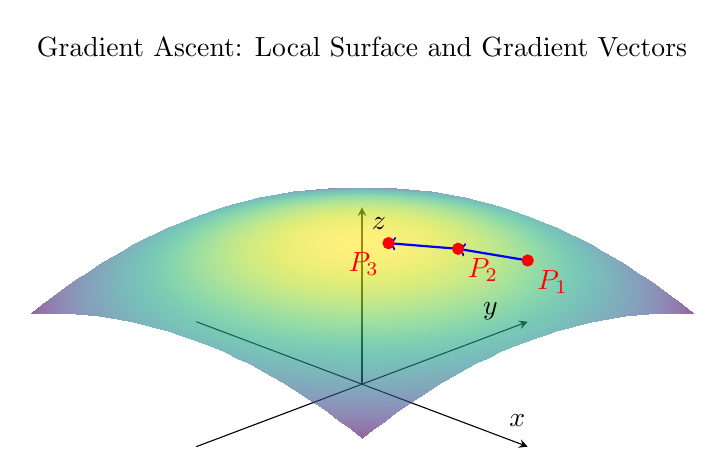
\begin{tikzpicture}
  \begin{axis}[
    view={45}{45},
    xlabel={$x$}, ylabel={$y$}, zlabel={$z$},
    domain=-1:1,
    y domain=-1:1,
    zmin=0, zmax=5,
    grid=major,
    samples=30,
    samples y=30,
    colormap/viridis,
    title={Gradient Ascent: Local Surface and Gradient Vectors},
    axis lines=center,
    ticks=none,
    width=10cm, height=7cm,
  ]
    \addplot3[surf, opacity=0.6, shader=interp] {4 - x^2 - y^2};
    \addplot3[only marks, mark=*, mark size=2pt, color=red]
      coordinates {(0.5, 0.5, 3.5) (0.29, 0.29, 3.83) (0.08, 0.08, 3.99)};
    \addplot3[->, thick, blue] coordinates {(0.5, 0.5, 3.5) (0.29, 0.29, 3.83)};
    \addplot3[->, thick, blue] coordinates {(0.29, 0.29, 3.83) (0.08, 0.08, 3.99)};
    \node[below right, red] at (axis cs:0.5,0.5,3.5) {$\vect{P}_1$};
    \node[below right, red] at (axis cs:0.29,0.29,3.83) {$\vect{P}_2$};
    \node[below left, red] at (axis cs:0.08,0.08,3.99) {$\vect{P}_3$};
  \end{axis}
\end{tikzpicture}\\
{\small Gradient ascent on $f(x,y)=4-x^2-y^2$. Starting at $\vect{P}_1$, each step moves in the direction of $+\nabla f$, climbing toward the maximum at the origin. Gradient descent (to minimize) uses $-\nabla f$ instead.}
\end{center}

%=============================================================
\wsection{Gradient Ascent and Descent}

\begin{formulabox}{Gradient Descent Algorithm}
To minimize $f(\vect{x})$:
\begin{enumerate}[nosep]
  \item \textbf{Compute} $\nabla f(\vect{p}_n)$
  \item \textbf{Unit direction:} $\uvec{d} = -\frac{\nabla f}{\|\nabla f\|}$ (steepest decrease)
  \item \textbf{Update:} $\vect{p}_{n+1} = \vect{p}_n + \eta\,\uvec{d} = \vect{p}_n - \eta\,\frac{\nabla f(\vect{p}_n)}{\|\nabla f(\vect{p}_n)\|}$
  \item \textbf{Iterate} until convergence
\end{enumerate}

For \textbf{gradient ascent} (maximize), use $+\nabla f$ instead.
\end{formulabox}

\begin{example}[Gradient Descent on $f = x^2 + 4y^2$]
Minimize $f(x,y) = x^2 + 4y^2$ starting from $\vect{p}_0 = (4, 2)$ with step size $\eta = 0.5$. Do 3 iterations.

$\nabla f = \vec{2x, 8y}$

\wbbox{
\textbf{Iteration 1:} $\nabla f(4,2) = \vec{8, 16}$, \; $\|\nabla f\| = \sqrt{64+256} = 8\sqrt{5}$

$\vect{p}_1 = (4,2) - \frac{0.5}{8\sqrt{5}}\vec{8,16} = (4,2) - \vec{0.224, 0.447} \approx (3.776, 1.553)$

$f(\vect{p}_1) \approx 14.26 + 9.65 = 23.9$ \; (down from $f(\vect{p}_0) = 32$)

\medskip
\textbf{Iteration 2:} $\nabla f(3.776, 1.553) \approx \vec{7.55, 12.42}$, \; $\|\nabla f\| \approx 14.53$

$\vect{p}_2 \approx (3.776, 1.553) - \frac{0.5}{14.53}\vec{7.55, 12.42} \approx (3.516, 1.126)$

$f(\vect{p}_2) \approx 12.36 + 5.07 = 17.4$

\medskip
\textbf{Iteration 3:} $\nabla f(3.516, 1.126) \approx \vec{7.03, 9.01}$, \; $\|\nabla f\| \approx 11.43$

$\vect{p}_3 \approx (3.516, 1.126) - \frac{0.5}{11.43}\vec{7.03, 9.01} \approx (3.209, 0.732)$

$f(\vect{p}_3) \approx 10.30 + 2.14 = 12.4$

Each iteration decreases $f$: $32 \to 23.9 \to 17.4 \to 12.4$, converging toward the minimum at $(0,0)$.
}{8cm}
\end{example}

\begin{example}[Gradient Ascent on $f = -x^2 - y^2 + 4x + 4y$]
Maximize $f(x,y) = -x^2 - y^2 + 4x + 4y$ starting from $\vect{p}_0 = (0,0)$ with $\eta = 0.5$. Do 3 iterations.

$\nabla f = \vec{-2x+4,\; -2y+4}$

\wbbox{
\textbf{Iteration 1:} $\nabla f(0,0) = \vec{4,4}$, \; $\|\nabla f\| = 4\sqrt{2}$

$\vect{p}_1 = (0,0) + \frac{0.5}{4\sqrt{2}}\vec{4,4} = \left(\frac{1}{2\sqrt{2}}, \frac{1}{2\sqrt{2}}\right) \approx (0.354, 0.354)$

$f(\vect{p}_1) \approx -0.125 - 0.125 + 1.414 + 1.414 = 2.58$ \; (up from $f(\vect{p}_0) = 0$)

\medskip
\textbf{Iteration 2:} $\nabla f(0.354, 0.354) = \vec{3.29, 3.29}$, \; $\|\nabla f\| \approx 4.65$

$\vect{p}_2 \approx (0.354, 0.354) + \frac{0.5}{4.65}\vec{3.29, 3.29} \approx (0.708, 0.708)$

$f(\vect{p}_2) \approx -0.501 - 0.501 + 2.832 + 2.832 = 4.66$

\medskip
\textbf{Iteration 3:} $\nabla f(0.708, 0.708) = \vec{2.58, 2.58}$, \; $\|\nabla f\| \approx 3.65$

$\vect{p}_3 \approx (0.708, 0.708) + \frac{0.5}{3.65}\vec{2.58, 2.58} \approx (1.061, 1.061)$

$f(\vect{p}_3) \approx 5.88$

Converging toward the maximum at $(2,2)$ where $f(2,2) = 8$: \; $0 \to 2.58 \to 4.66 \to 5.88$.
}{8.5cm}
\end{example}

\wsubsection{Connection to Machine Learning}

-- In ML, a model has parameters $\vect{w}$ and a \textbf{loss function} $L(\vect{w})$ measuring error

-- Training = gradient descent on $L$: $\vect{w}_{n+1} = \vect{w}_n - \eta\,\nabla L(\vect{w}_n)$

-- The step size $\eta$ is called the \textbf{learning rate}

-- This is how neural networks, logistic regression, and most modern AI models are trained

%=============================================================

\begin{practice}

\prob Find $\nabla f$ for $f(x,y) = xe^y + \sin(xy)$ at the point $(0, \pi)$.

\wbbox{
$\nabla f = \vec{e^y + y\cos(xy),\; xe^y + x\cos(xy)}$. At $(0,\pi)$: $\nabla f = \vec{e^\pi + \pi, 0}$.
}{2.5cm}

\wans{$\nabla f(0,\pi) = $ \wbml{$\vec{e^\pi + \pi,\; 0}$}}

\vspace{2.5cm}

\prob Find the maximum rate of change of $f(x,y,z) = \sqrt{x^2+y^2+z^2}$ at $(3,4,12)$ and the direction in which it occurs.

\wbbox{
$\nabla f = \frac{1}{\sqrt{x^2+y^2+z^2}}\vec{x,y,z}$. At $(3,4,12)$: $f = 13$.

$\nabla f = \frac{1}{13}\vec{3,4,12}$. Max rate $= \|\nabla f\| = 1$. Direction: $\frac{1}{13}\vec{3,4,12}$.
}{3cm}

\vspace{3cm}

\prob Find the directional derivative of $f(x,y) = x^2 - 3y^2$ at $(2, -1)$ in the direction toward the point $(5, 3)$.

\wbbox{
Direction: $\vec{5-2, 3-(-1)} = \vec{3,4}$, $\uvec{u} = \vec{3/5, 4/5}$.

$\nabla f = \vec{2x, -6y}$. At $(2,-1)$: $\nabla f = \vec{4, 6}$.

$D_{\uvec{u}}f = \vec{4,6}\cdot\vec{3/5, 4/5} = 12/5 + 24/5 = 36/5$.
}{3.5cm}

\vspace{3cm}

\prob Perform 2 iterations of gradient descent on $f(x,y) = (x-3)^2 + (y+1)^2$ from $\vect{p}_0 = (0,0)$ with $\eta = 1$.

\wbbox{
$\nabla f = \vec{2(x-3), 2(y+1)}$

Iteration 1: $\nabla f(0,0) = \vec{-6, 2}$, $\|\nabla f\| = \sqrt{40} = 2\sqrt{10}$.

$\vect{p}_1 = (0,0) - \frac{1}{2\sqrt{10}}\vec{-6, 2} = \left(\frac{3}{\sqrt{10}}, -\frac{1}{\sqrt{10}}\right) \approx (0.949, -0.316)$

$f(\vect{p}_1) \approx (0.949-3)^2 + (-0.316+1)^2 = 4.21 + 0.47 = 4.68$ (down from 10)

Iteration 2: $\nabla f(0.949, -0.316) = \vec{-4.10, 1.37}$, $\|\nabla f\| \approx 4.32$

$\vect{p}_2 \approx (0.949,-0.316) - \frac{1}{4.32}\vec{-4.10, 1.37} \approx (1.898, -0.633)$

$f(\vect{p}_2) \approx 1.21 + 0.13 = 1.35$ (converging toward min at $(3,-1)$)
}{6cm}

\wans{$\vect{p}_2 \approx $ \wbml{$(1.90, -0.63)$}}

\vspace{3cm}

\prob Show that $\nabla f$ is perpendicular to level curves. \textit{Hint:} If $\vect{r}(t)$ is a curve on the level surface $f=k$, differentiate $f(\vect{r}(t))=k$.

\wbbox{
$\frac{d}{dt}[f(\vect{r}(t))] = \frac{d}{dt}[k] = 0$

By the chain rule: $\nabla f(\vect{r}(t)) \cdot \vect{r}\,'(t) = 0$

Since $\vect{r}\,'(t)$ is tangent to the level curve, this says $\nabla f \perp$ the level curve. $\square$
}{3cm}

\end{practice}

\end{document}
